\documentclass[10pt]{article} %%%%%%%%%%%%%%%%%%%%%%%%%%%
%%%%%%%%%%%%%%%%%%%%%%%%%%%%%%%%%%%%%%%%%%%%%%%%%%%%%%%%%
%%%
%%% Apsrtable writeup for TPM, coinciding with 0.7-0
%%%
%%% mjm / 2009-01-14 %%%%%%%%%%%%%%%%%%%%%%%%%%%%%%%%%%%%


\usepackage[dvipsnames,usenames]{xcolor}
\usepackage[opticals,medfamily,minionint,footnotefigures]{MinionPro}
\usepackage[no-math]{fontspec}
\usepackage{xltxtra}
\usepackage[protrusion=true,expansion]{microtype}
%%% Hanging indents: args length, number of lines.
%%% \begin{hangparas}{1em}{1}
\usepackage{hanging} 
%%% Date formatting, defn of isodate
\usepackage{datetime}
\renewcommand{\dateseparator}{-}
\newdateformat{isodate}{%
\THEYEAR\dateseparator\twodigit{\THEMONTH}\dateseparator\twodigit{\THEDAY}}


%%% Set up bold Minion Pro math
\usepackage{bm}
 \DeclareMathAlphabet\mathbf {T1} {MinionPro-OsF}{b}{n}
 \SetMathAlphabet\mathit  {bold}{T1} {MinionPro-OsF}{b}{it}
 \SetSymbolFont{operators}{bold}{T1} {MinionPro-OsF}{b}{n}
 \SetSymbolFont{letters}  {bold}{OML}{MinionPro-TOsF} {b}{it}
\DeclareMathVersion{boldtabular}
\SetSymbolFont{operators}{boldtabular}{T1} {MinionPro-OsF}{b}{n}
\SetSymbolFont{letters}  {boldtabular}{OML}{MinionPro-TOsF}  {b}{it}
\SetMathAlphabet\mathit  {boldtabular}{T1} {MinionPro-OsF}{b}{it}
\DeclareMathAlphabet\mathebf {T1} {MinionPro-OsF}{eb}{n}

%%% PDF setup -- fill in the title
\usepackage[dvipdfm, bookmarks, colorlinks, breaklinks, pdftitle={Malecki},pdfauthor={Michael Malecki}]{hyperref}  
\hypersetup{linkcolor=NavyBlue,citecolor=NavyBlue,filecolor=NavyBlue,urlcolor=NavyBlue} 

%% Alter some LaTeX defaults for better treatment of figures:
%% This is from the first result of google: "latex dumb defaults"
    \renewcommand{\topfraction}{0.9}	
    \renewcommand{\bottomfraction}{0.8}	
    %   Parameters for TEXT pages (not float pages):
    \setcounter{topnumber}{2}
    \setcounter{bottomnumber}{2}
    \setcounter{totalnumber}{4}     
    \setcounter{dbltopnumber}{2}    
    \renewcommand{\dbltopfraction}{0.9}	
    \renewcommand{\textfraction}{0.07}	
    %   Parameters for FLOAT pages (not text pages):
    \renewcommand{\floatpagefraction}{0.7}	% require fuller float pages
	% N.B.: floatpagefraction MUST be less than topfraction !!
    \renewcommand{\dblfloatpagefraction}{0.7}	% require fuller float pages

%%% Enable the bibliography
%%%     see  http://merkel.zoneo.net/Latex/natbib.php
%%% 
%%% round: use () for in-text cites (other options square, curly, angle)
%%% sort: orders multiple citations into the sequence in which they 
%%%       appear in the list of references;
%%% sort&compress: as sort but in addition multiple numerical
%%%                citations are compressed if possible (as 3-6, 15);
%%% numbers: for numerica citations
%%% super:   superscripted numbers as in Nature
\usepackage[round]{natbib}
%%% Want to change the section head of the bib??
%\AtBeginDocument{\renewcommand\refname{LITERATURE CITED}}

%%% Document layout, margins
\usepackage{geometry} 
\geometry{letterpaper, textwidth=6.5in, textheight=8in, marginparsep=1em}

%%% This is how you set  line spacing globally inside []
%%% Options are "singlespacing","onehalfspacing","doublespacing"
%%% To change WITHIN the document (you want a section single spaced)
%%% just drop in, where needed, \singlespacing
%%% and then \doublespacing again when finished.
\usepackage[onehalfspacing]{setspace} 

%\usepackage{egameps} % See Martin Osborne's documentation!
%\usepackage{sgame} % See Osborne
%\usepackage{hyperref} % \href{http://link.com}{link text} DEF EARLIER
\usepackage{graphicx} % for figures of all kinds

%% Caption labels bold. Always left-align, do not center short ones.
%% Use . instead of : after label. Size option.
\usepackage[bf,nooneline,labelsep=period,footnotesize]{caption}
\usepackage{dcolumn}  % enable decimal align tables
%\usepackage{wrapfig}  % wrappable figures

%%% How to treat new paragraphs: units are anything that latex
%%% understands: in, mm, pt, cm, [em, ex (typographic units!)]
\setlength{\parindent}{1em} % 1em  indent first line
\setlength{\parskip}{0.5ex} % half x-height space between para

%%% Working Example of how you specify shortcut macros:
\newcommand{\ybar}{\ensuremath{\overline{y}}}

%%% Other options: Options>Soft wordwrap for easy viewing
%%% Italics and Bold: ctrl+C,F,I (C-c, C-f, C-i) for inserting italicized text. 
%%% CFB for bold.
%%% rm sf tt md bf up it sl sc 
%%% Drag citations from Bibdesk
%%% single - for intraword hyphen. Anything longer, use two -- or three ---

%%% Figures. Wrapfigure at Right Left or Center.
%%% Set bounding box size (same as figure size).
%%% Insert your figure BEFORE the text. 
%%% Subsequent text will wrap around the figure.

%%% Normally, just use figure environment.
%%% To insert a figure, drag the icon (without typing the command!) 
%%% from the finder and it will insert.
%%% Type width= or height= in the [options] before the {argument}.
%%% Latex>Insert Envt>Figure (figure* means no number)
%%% "Figure #." is handled by latex, not you. Just type.
%%% To refer to a figure (or any \label) type \ref{thelabel}
%%% in text or use Ref menu, "C-c )" emacs will do it for you.



%%% FONTS

% converts LaTeX specials (``quotes'' --- dashes etc.) to unicode
\defaultfontfeatures{Ligatures={Common}} 
%\setromanfont [Mapping=tex-text,Ligatures={Common}, BoldFont={* Bold}, ItalicFont={* Italic}]{Gentium Book Basic}
\setmainfont [Mapping=tex-text,Ligatures={Common},BoldFont={ElectraLH-Bold},ItalicFont={ElectraLH-CursiveOsF},BoldItalicFont={ElectraLH-BoldCursiveOsF},SmallCapsFont={ElectraLH-RegularSC}]{ElectraLH-RegularOsF}
\setsansfont[Mapping=tex-text,BoldFont={Delicious-Bold},ItalicFont={Delicious-Italic},SmallCapsFont={Delicious-SmallCaps}] {Delicious-Roman}
\setmonofont[Scale=0.8]{Monaco} 
%%% Section headings
\usepackage{sectsty} 
\usepackage[normalem]{ulem} 
\sectionfont{\sffamily\mdseries\upshape\Large}
\subsectionfont{\sffamily\bfseries\upshape\normalsize} 
\subsubsectionfont{\sffamily\mdseries\upshape\normalsize} 
%%% Hang section numbers in the left margin
\makeatletter 
\def\@seccntformat#1{\protect\makebox[0pt][r]{\csname 
the#1\endcsname\quad}} 
\makeatother 
\usepackage{Sweave}
%\VignetteIndexEntry{Using and Extending apsrtable}
\begin{document}


\title{Replicable Publication-Ready Model Output with R package apsrtable\\Implementation \& Extension Guide}
\author{\href{http://malecki.wustl.edu}{Michael Malecki}\footnote{PhD Candidate, Washington University in St. Louis}}
\maketitle

\section{Overview}
\label{sec:overview}

Formatting fitted model objects is not trivial and should not be done at the last minute before submitting a paper. It is too easy for modeling details to get lost, or simply for values to be omitted, transposed, or otherwise misplaced. Thus automation is a boon, if not a requirement, for replicability.

Fitted model objects in R contain a lot of information, but often we want to look at several of them side-by-side. It would be nice to name the models, and include some model-fit information, and to name the covariates. Nested and non-nested models and naming become a problem for cbind and rbind, and last but not least, we want this information in some legible format -- either plain text or, prefereably, Latex. My R package \textit{apsrtable}, installable from \href{http://cran.r-project.org/web/packages/apsrtable/index.html}{CRAN}, seeks to solve all of these problems, creating tables ready to be published in the \textit{APSR}. I might have named it after \textit{Political Analysis}, but the latter often features other innovative presentations of data and results, such that ``a \textit{PA}-style table'' is less identifiable.

Like many graduate students -- including probably most who read TPM -- I have typeset \emph{a lot} of fitted models in the course of methods training, leaving aside the relatively few tables that make their way into final seminar, conference, or journal papers. We were ``strongly encouraged'' to prepare homework assignments using Latex and create ``professional-looking'' tables of model output, with the expectation that we would get faster at it, while becoming attuned to the intricacies of Latex's tabular and matrix environments. I found this exercise as tedious as formatting a bibliography by hand. So, I set out to automate R's output of ``professional-looking'' tables. To complete the bibliography analogy, I also wanted to make the automated solution more user-friendly than bibtex BSTs -- though ``an order of magnitude easier than BST'' is still an extremely low target.

\section{Usage}
\label{sec:usage}

To demonstrate \texttt{apsrtable}'s features, I'll replicate some of the results from Persson and Tabellini's (2003) \textit{The Economic Effects of Constitutions}\footnote{The data are available from the \href{http://www.igier.unibocconi.it/whos.php?vedi=1169&tbn=albero&id_folder=177}{authors}, though they may contain some coding errors in the institutional interaction variables. A corrected replication dataset is available \href{http://malecki.wustl.edu/pt.csv}{here}.}, in particular models 1--3 of Table 6.1 (p.~159) (Figure \ref{fig:ptimage}).
\begin{figure}[htb]
  \centering
  \caption{Persson and Tabellini (2003), p.159, detail.}
  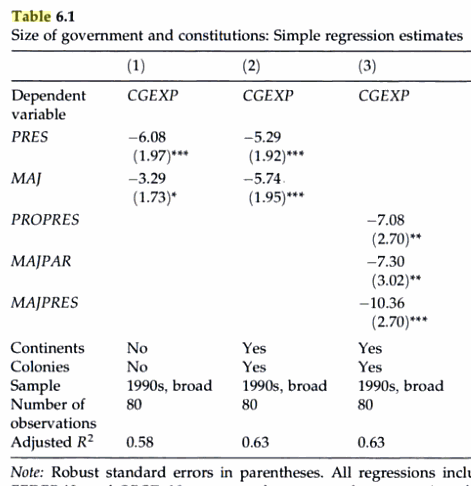
\includegraphics[width=8cm]{pt-table.png}
  \label{fig:ptimage}
\end{figure}
\begin{Schunk}
\begin{Sinput}
> pt <- read.csv("pt.csv")
> library(apsrtable)
> controls <- "lyp + gastil + age + trade + prop65 + prop1564 + federal + oecd"
> regions <- "col_uka + col_espa + col_otha + africa + asiae + laam"
> model1 <- lm(as.formula(paste("cgexp ~", paste(c("pres + maj",
                                                  controls),collapse="+"))), data=pt)
> model2 <- lm(as.formula(paste("cgexp ~",paste(c("pres + maj",
                                                 controls,regions),collapse="+"))), data=pt)
> model3 <- lm(as.formula(paste("cgexp ~",paste(c("pro.pres + maj.parl + maj.pres",
                                                 controls,regions),collapse="+"))), data=pt)
\end{Sinput}
\end{Schunk}

The result of simply calling \texttt{apsrtable(model1, model2, model3)} shouldn't be very far from usable output. We get decimal-aligned columns that are also lined up in the Latex source, errors in parentheses, and a single star indicating $p<.05$. But, we want to include ``robust'' standard errors, omit a bunch of controls, give the variables less cryptic names, and, to complete the exercise, add more stars. All of these are extremely easy to do with \emph{apsrtable}, but looking at the default output is a helpful baseline and a recommended first step every time.
\begin{description}
\item[Alternate Standard Errors] However you want to go about estimating alternative standard errors, simply insert a vector or the full new variance-covariance matrix into the fitted model object and name it \texttt{se}\footnote{Most model objects are simply lists rather than formal classes (that is, they use the S3 class system). Models fit with \texttt{lmer} are formally \textit{mer} class objects but changes in how \textit{lme4} methods \texttt{display} and \texttt{summary} work has prevented incorporation of that class of models so far.} To get the same standard errors that Persson and Tabellini report (also, I believe, the Stata default), use the \textit{sandwich} package:\\ \verb|model1$se <- vcovHC(model1,type="HC1")| and so on for each model. By default, apsrtable will include only the robust standard errors when present, but the argument \texttt{se} can either ignore them and print the model's original standard errors (``vcov'') or both (``both'').
\item[Order of Covariates] Including nested and non-nested models side-by-side, lining up the covariates that are included and leaving blank those that are not, is the main feature of the package. For this replication (and most of the time) the default ``lr'' left-to-right incorporation of terms is correct. For special cases, two other options, ``rl'' and ``longest'' are provided and discussed briefly under implementation details. For typical use, it is best to nail down the desired order in which the models are passed to the function, and then the value of \verb|order|.
\item[Omitting controls] Variables can be omitted from the display either by name or index. It is easiest in this case to supply the argument \verb|omit=c(1,4:17)|. However, the order of coefficients can change, so a list of quoted character names of coefficients to omit may be safer, and certainly makes your code more transparent and thus easier to maintain and replicate. As of version 0.8, you can also provide an \verb|expression|, such as a regular expression. In this case, the argument should take the form:\\
  \verb|expression(grep(pattern,coefnames))|\\
  The internal object \verb|coefnames| is the ordered union of all terms in all models. 
  
  To include multiple regular expressions, or a mix of expressions with
  other types, you may supply a \verb|list|, but you must ensure that
  the result is a valid subscript list: all character, all numeric, or
  all logical. For example, if you refer to a specific coefficient by
  its character name, include the argument \verb|value=TRUE| in any
  \verb|grep| expressions in the list.
\item[Names of Models and Covariates] Models by default are named ``Model 1'', ``Model 2'', etc., but numbering can be changed arbitrarily (via argument \verb|model.counter|), or a vector of meaningful names can be supplied as \verb|model.names| (if it comes up short, numbering accounts for the named ones).

Covariate name replacement takes place after the list of included coefficients from all the models has been generated. Therefore, again it is a good idea to look at the default, settle on the values of \verb|order| and \verb|omitcoef|, and only then supply a vector of coefficient display names as the argument \verb|coef.names|.
\item[Stars] The default behavior is to indicate coefficient significance at the level $p<.05$ with a single superscript asterisk. Two arguments allow you to increase the sparkle of almost any table. To set a different level for a single star, supply it to \verb|lev|. To include a dagger for .10, a star for .05, two stars for .01, and three stars (!) for .001, supply the argument \verb|stars="default"|. I admit the name is confusing, but ``default'' here indicates the R default rather than the APSR and \textit{apsrtable} default.
\item[Other arguments] The other arguments are documented in the package, but two are worth mention here. The handling of notes about standard errors and significance indicators is discussed below. Also, \verb|Sweave=TRUE| should be used whenever you include a call to \verb|apsrtable| from within a Sweave document. Otherwise output will include the table environment code and empty caption and label, which should be included in the Sweave document itself if emacs reftex is to keep track of tables. An internal test for Sweave might appear in future versions, but the default output is meant for cutting and pasting from an R session into a Latex document, which seems to be fairly common workflow.
\end{description}

\section{Some Implementation Details}
\label{sec:implementation}
Three features of \textit{apsrtable} bear mention for how I implemented them: covariate aggregation across models, table notes, and model summaries, which provides a flexible extension framework.

\subsection{Covariate Order}
\label{sec:covariate-order}


Authors have immense control over the order in which covariate rows are presented in the final table. Through a combination of the order of terms in the model objects, and the choice of \verb|order| in the call to \verb|apsrtable|, one should be able to create tables that never need ``rearrangement'' of rows between output and publication. First, it builds a list of all variable names, and then notes the position of the variables in each model with respect to this final order. Next, the \verb|omitcoef| list is marked, and finally, the names of remaining terms are replaced with the optional list of \verb|coef.names|, which, of course, may contain Latex
 markup. The column of variable names is set in text mode, so any math should be delimited by \$, and because it's R, backslashes have to be doubled. A label ``$\beta_0$ Intercept'' would be supplied as \verb|"$\\beta_0$ Intercept"|.

The default left-to-right order starts with the first model; any terms included in the second not in the first are appended to the order, and so on. Right-to-left (\verb|order="rl"|) takes the initial order from the rightmost model; and \verb|order="longest"| starts with the order of terms in the model with the most terms, wherever it is in the list of models, then appends any others always left-to-right.

\subsection{Table Notes}
\label{sec:table-notes}

Some kinds of notes pertaining to the table depend on values used to generate it. In particular, informing readers of ``robust'' standard errors, and the indicators and ``level'' of statistical significance lies in the gap between content and presentation. Authors also commonly indicate the source of data in a note beneath a table (technically a multicolumn span within the tabular environment). 

The \verb|notes| argument allows you to specify a list of functions or character strings. R's ``lazy evaluation'' means that these functions are evaluated only when \verb|eval| is called explicitly inside \verb|apsrtable|. R's variable scoping meant that the variables in the \verb|apsrtable()| call reside 3 levels up the call stack, so custom functions in the \verb|notes| list can only access them by specifying the environment at \verb|sys.frame(-3)|. Of course, simple character strings are valid in the \verb|notes| list and will be typset along with the results of the dynamic functions.

\subsection{Extending apsrtable with \texttt{modelInfo}}
\label{sec:modelinfo}



Besides the coefficients, standard errors, and statistical significance star(s), model summaries and some indication of goodness-of-fit should be included with each model, which I call \textit{modelInfo}. But, different researchers prefer to include different statistics describing models as a whole. Therefore, \textit{apsrtable} comes with some reasonable defaults and a simple mechanism to change them. The same mechanism makes extending the package to other types of models relatively easy.

ModelInfo methods are called on the list of model summaries (that is, the result of \verb|summary(model)|). At a minimum, one can select from the information contained therein to generate a list of named character strings that comprise the modelInfo that will be included in the final output. The formatter doesn't care what you include here -- it simply matches the names (always left-to-right) across models and prints it all. If the \verb|summary| object does not contain some data that you need for a model summary statistic, see Section \ref{sec:extend-other-models} for creating special \texttt{apsrtableSummary} methods that return the information you want.

So, what does a modelInfo method look like? It is a formal S4 method that takes a model summary object as its argument. Therefore to change the list of model information, just change what the modelInfo function returns for a given model class. Future versions will probably include a selection of presets, but changing by a quick call to \verb|setMethod| is straightforward and my aim here is to make clear how to get the modelInfo you want. For \verb|lm| objects, the default prints the $N$, $R^2$, adjusted $R^2$, and residual sd. The example in \verb|?modelInfo| shows you how to print only the $N$ and residual sd; the easiest way to find the default is via \verb|getMethod("modelInfo","summary.lm")|. The defaults for \verb|lm| and \verb|glm| are also included as named private functions, to make reversion easier (see the modelInfo example).

To return to the Persson and Tabellini example, they summarize the controls used (but not displayed) in the modelInfo section. It is simple to write a function for \verb|summary.lm| that tests for the presence of a particular name among coefficients. Besides this, they report the $N$ as ``Number of Observations'' (so we want to change the name of that element in the list), and the adjusted $R^2$. So, we just create a custom \verb|modelInfo| method that returns these items.
\begin{Schunk}
\begin{Sinput}
> ## Add robust se to the models
> library(sandwich)
> model1$se <- vcovHC(model1,type="HC1")
> model2$se <- vcovHC(model2,type="HC1")
> model3$se <- vcovHC(model3,type="HC1")
> ## Create and register custom modelInfo for lm
> 
> setMethod("modelInfo", "summary.lm", function(x) {
   env <- parent.frame()
   digits <- evalq(digits,env)
   model.info <- list(
     "Continents"= (
         ifelse(!is.na(charmatch("laam",rownames(coef(x)))),
           "\\multicolumn{1}{c}{Yes}", "\\multicolumn{1}{c}{No}")),
     "Colonies" = (
         ifelse(!is.na(charmatch("col",rownames(coef(x)))),
           "\\multicolumn{1}{c}{Yes}", "\\multicolumn{1}{c}{No}")),
     "Number of\\tabularnewline Observations"= (formatC(sum(x$df[1:2]),format="d")),
     "adj. $R^2$" = (formatC(x$adj.r.squared,format="f",digits=digits)))
 class(model.info) <- "model.info"
 return(model.info)
 } )
\end{Sinput}
\end{Schunk}

With the new modelInfo method registered, the final call to \verb|apsrtable()| is shown below, and the results typeset as Table \ref{final-table}. Note that the \verb|omitcoef| list contains a character element and then two expressions that evaluate to character vectors.
\begin{Schunk}
\begin{Sinput}
> apsrtable(model1,model2,model3,
 omitcoef=list("(Intercept)", expression(strsplit(controls," \\+ " )), expression(strsplit(regions," \\+ "))),
 coef.names=c("Presidential","Majoritatian", 
   "Proportional Presidential", "Majoritarian Parliamentary", "Majoritarian Presidential"),
 align="left",stars="default",
 notes=list(se.note(), stars.note())
 )
\end{Sinput}
\end{Schunk}
\begin{table}[!ht]
\centering
\caption{Replication of Models 1--3 from Persson and Tabellini (2003), p. 149: ``Size of government and constitutions: Simple regression estimates.''}
\label{final-table}
\begin{tabular}{ l D{.}{.}{2}@{\hspace{3em}}D{.}{.}{2}@{\hspace{3em}}D{.}{.}{2} } 
\hline 
  & \multicolumn{ 1 }{ c }{ Model 1 } & \multicolumn{ 1 }{ c }{ Model 2 } & \multicolumn{ 1 }{ c }{ Model 3 } \\ \hline
 %                                      & Model 1                  & Model 2                  & Model 3                 \\ 
Presidential                           & -6.08 ^{**}              & -5.29 ^{**}              &                         \\ 
                                       & (1.97)                   & (1.92)                   &                         \\ 
Majoritatian                           & -3.29 ^\dagger          & -5.74 ^{**}              &                         \\ 
                                       & (1.73)                   & (1.95)                   &                         \\ 
Proportional Presidential              &                          &                          & -7.08 ^*                \\ 
                                       &                          &                          & (2.70)                  \\ 
Majoritarian Parliamentary             &                          &                          & -7.30 ^*                \\ 
                                       &                          &                          & (3.02)                  \\ 
Majoritarian Presidential              &                          &                          & -10.36 ^{***}           \\ 
                                       &                          &                          & (2.70)                   \\
 Continents                             & \multicolumn{1}{c}{No}  & \multicolumn{1}{c}{Yes} & \multicolumn{1}{c}{Yes}\\ 
Colonies                               & \multicolumn{1}{c}{No}  & \multicolumn{1}{c}{Yes} & \multicolumn{1}{c}{Yes}\\ 
Number of\tabularnewline Observations & 80                       & 80                       & 80                      \\ 
adj. $R^2$                             & 0.58                     & 0.63                     & 0.63                     \\ \hline
 \multicolumn{4}{l}{\footnotesize{Robust standard errors in parentheses}}\\
\multicolumn{4}{l}{\footnotesize{$^\dagger$ significant at $p<.10$; $^* p<.05$; $^{**} p<.01$; $^{***} p<.001$}} 
\end{tabular} \end{table}


The example above shows how the \verb|modelInfo| methods can be used to change the display for linear model summary objects. In theory, any model object for which \verb|coef|, \verb|vcov|, and \verb|summary| methods should work with \textit{apsrtable}. Extending means mainly creating \verb|modelInfo| methods for other classes of model summaries. 

\subsection{Adding model classes with \texttt{apsrtableSummary}}
\label{sec:extend-other-models}

Sometimes, the \texttt{summary} method for a given object either does not exist, or does not produce output that \emph{apsrtable} knows what to do with. In this case, users have two options: write a replacement summary method and submitting it to package maintainers, or create a summary method that only \textit{apsrtable} will use. Presumably, the latter may be a stopgap on the way to the former.

One user requested support for the \textit{gee} package, specifically \texttt{gee.robust} objects. A summary of them suitable for \textit{apsrtable} would have to place the “robust” standard errors into the \texttt{\$se} position of the summary object, as well as turn the \texttt{summary.gee}'s columns of $z$-scores into $\Pr(z)$ for the bedazzler \texttt{apsrstars}.\footnote{Relatedly, an \texttt{apsrtableSummary} may be needed just to \emph{rename} columns in some summary coefficient matricies. The function \texttt{apsrstars}, derived from \texttt{stats:::printCoefmat}, checks for column names starting with “$\Pr($”.} The solution is to write a replacement \texttt{apsrtableSummary} which is always tried first, with the model-object's default \texttt{summary} called otherwise.

The example manipulates the output of \texttt{summary.gee} into a matrix (and \texttt{\$se} vector) suitable for seamless use with \textit{apsrtable.}
\begin{Schunk}
\begin{Sinput}
> "apsrtableSummary.gee" <- function(x) {
   s <- summary(x)
   newCoef <- coef(s)
   ## which columns have z scores? (two of them in robust case)
   zcols <- grep("z",colnames(newCoef))
   newCoef[,zcols] <- pnorm(abs(newCoef[,zcols]), lower.tail=FALSE)
   colnames(newCoef)[zcols] <- "Pr(z)"
   s$coefficients <- newCoef
   ## put the robust se in $se so that notefunction works automatically
   ## the se checker will overwrite [,4] with pt, but this doesn't matter
   ## because the last column Pr(z) is used by apsrstars() anyway
   ## and the se are pulled from $se.
   if( class(x)[1] == "gee.robust") {
     s$se <- coef(s)[,4]
   }
   return(s)
 }
\end{Sinput}
\end{Schunk}


\section{Conclusion}
\label{sec:extending-apsrtable}
I saw a striking need to produce publication-ready output as a part of the modeling process, especially as complexity grew. Not surprisingly, I learned after publishing the package on CRAN and announcing it to PolMeth, that I was not alone. Martin Elff has a similar function (\verb|mtable|) in his \textit{memisc} package, which can also produce non-Latex output. Some of the details of his implementation caused me to refactor parts of my own. My current workflow relies heavily on Sweave to  ensure that the code I run is actually connected to both the theoretical arguments I make and the results I present. I rely on \textit{apsrtable} to produce reliable, replicable, relatively painless tables of results. I hope that \textit{TPM} readers can save themselves (and their graduate students!) some typesetting frustration by using \textit{apsrtable}, and I look forward to extensions and improvements that users may provide.


\end{document}
